\documentclass{standalone}
\usepackage{tikz}
\usetikzlibrary{intersections, calc}
\usepackage{hsbcommon}
    \begin{document}
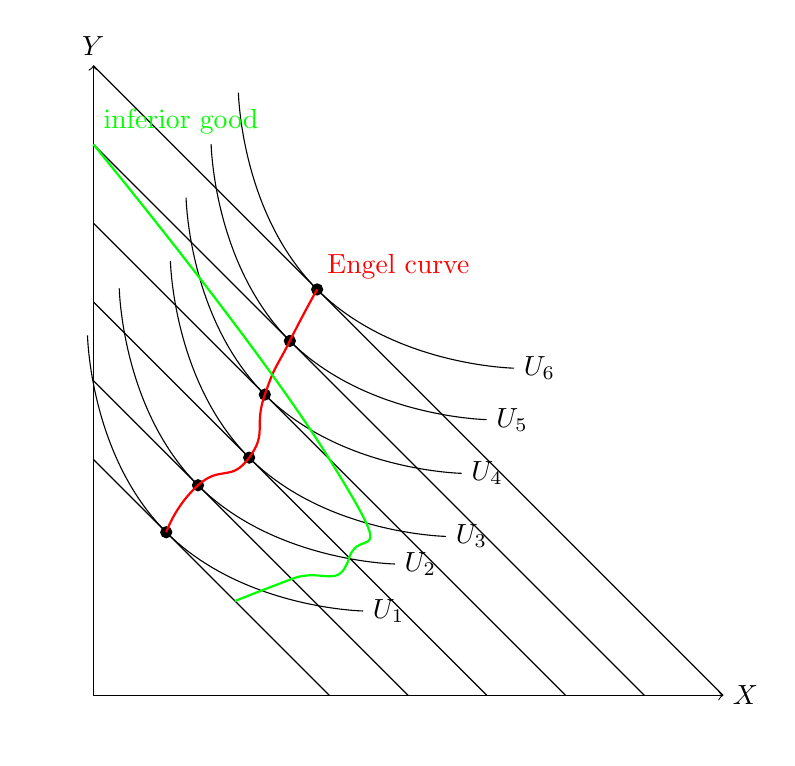
\begin{tikzpicture}
        \draw[->] (0,0) node[below] {\phantom{$X_i$}} -- (8,0) node[right]  {$X$};
        \draw[->] (0,0) node[left] {\phantom{$Y_mi$}} -- (0,8) node[above]  {$Y$};

        \def\mya{A}
        \def\myb{B}
        \def\mys{S}
        \def\myp{P}
        \def\myq{Q}
        \pgfmathsetseed{3}

        \foreach [count=\i] \x/\y/\mycolor/\myopacity in {3/3/black/1%
            ,4/4/black/1%
            ,5/5/black/1%
            ,6/6/black/1%
            ,7/7/black/1%
            ,8/8/black/1%
            }
        {       
                \begin{scope}[color=\mycolor,opacity=\myopacity]
                    \pgfmathsetmacro\mymove{rnd*(0.1)+0.3}
                    \coordinate (\mya) at (0,\y);
                    \coordinate (\myb) at (\x,0);
                    % \node[above right] at (\myb) {$B_\i$};
             
                    \draw [name path=budgetgerade\i] plot [smooth] coordinates {(\mya) (\myb) };
            
                    \coordinate (\mys\i) at ($(\mya)!\mymove!(\myb)$);  %% punkt (fast) in der mitte
                    
                    \filldraw (\mys\i) circle (2pt);
                    \coordinate (\myp) at ([shift=({-1cm,2.5cm})]\mys\i); %% punkt links oben
                    \coordinate (\myq) at ([shift=({2.5cm,-1cm})]\mys\i); %% punkt rechts unten
                    
                    \node[right] at (\myq) {$U_\i$};
            
                    \draw [name path=indifferenzkurve] plot [smooth, tension=1] coordinates {(\myp) (\mys\i) (\myq) };
                \end{scope}
        }        
                \ifstep{1}{
\begin{scope}[color=red]

                    \draw[thick] plot[smooth, tension=1] coordinates {(S1) (S2) (S3) (S4) (S5) (S6)}  node[above right] {Engel curve}  ;
                \end{scope}
}

                \ifstep{2}{
\begin{scope}[color=green]

                    \coordinate (P1) at ($(0,3)!0.6!(3,0)$);  
                    \coordinate (P2) at ($(0,4)!0.63!(4,0)$);  
                    \coordinate (P3) at ($(0,5)!0.65!(5,0)$);  
                    \coordinate (P4) at ($(0,6)!0.5!(6,0)$);  
                    \coordinate (P5) at ($(0,7)!0!(7,0)$);  
                                \draw[thick] plot[smooth, tension=1] coordinates {(P1) (P2) (P3) (P4) (P5)}  node[above right] {inferior good}  ;        
                \end{scope}
}

        
    \end{tikzpicture}
\end{document}
